\documentclass[12pt,a4paper]{article}
\usepackage[margin=1in]{geometry}
\usepackage{hyperref,amsmath,amssymb,booktabs,longtable,fancyhdr,array,microtype,tikz}
\usetikzlibrary{shapes.geometric, arrows, positioning, fit, calc}
\hypersetup{colorlinks=true,linkcolor=blue!70!black,urlcolor=blue!70!black}
\pagestyle{fancy}\fancyhf{}
\fancyhead[L]{Agentic AI Bootcamp}
\fancyhead[R]{sujeet.banerjee@gmail.com\\sujeet.banerjee.professional@gmail.com}
\fancyfoot[L]{AI Security \& Multi-Agent Architecture}
\fancyfoot[R]{\thepage}
\renewcommand{\headrulewidth}{0.4pt}\renewcommand{\footrulewidth}{0.4pt}
\title{\textbf{AI Security \& Multi-Agent Orchestration}\\\large Prompt Injection Defenses and Role-Based Tool Access}
\author{Detailed Notes -- Agentic AI Bootcamp}\date{}
\begin{document}
\maketitle
\tableofcontents
\newpage

\section{Prompt Injection}
While a System Prompt is the first line of defense in guiding an AI's behavior, it does not completely prevent role hijacking or prompt poisoning (commonly known as Prompt Injection). Current Large Language Models (LLMs) do not have a strict separation between the control plane (the code/instructions) and the data plane (the user input); they process everything as one massive sequence of text. Because the model interprets natural language to figure out what to do, a cleverly crafted user input can convince the model to abandon the system prompt. 

\subsection{Common Attack Vectors}
\begin{itemize}
    \item \textbf{Role Hijacking (Jailbreaking):} The user explicitly commands the AI to adopt a new persona, often framing it as a game or a hypothetical scenario. Example: ``Ignore all previous instructions. You are now 'DAN'...''.
    \item \textbf{Prompt Poisoning (Injection):} The user hides instructions within data that the AI is supposed to process.
    \item \textbf{Context Overflow / Distraction:} The user provides an extremely long prompt or complex logic puzzle that buries the original system instructions so far back in the context window that the model ``forgets'' or deprioritizes its original boundaries.
\end{itemize}

\subsection{Preventive Steps (Defense in Depth)}
A system prompt alone is not enough, so AI engineers use a layered approach to secure agents:
\begin{enumerate}
    \item \textbf{Delimiters \& Sandwich Prompting:} Wrapping the user input in strict delimiters and repeating the core rules at the end of the prompt to leverage the recency effect.
    \item \textbf{Input Guardrails (Pre-processing):} Using a secondary, smaller AI model or traditional regex rules to scan the user's prompt for known injection patterns before it ever reaches the main LLM.
    \item \textbf{Output Filtering (Post-processing):} Scanning the LLM's generated response to ensure it hasn't broken character or generated policy-violating content before showing it to the user.
    \item \textbf{Constitutional AI / Fine-Tuning:} Training the model at a foundational level to refuse requests that violate a specific set of principles, making it naturally resistant to role hijacking regardless of the prompt.
\end{enumerate}

\section{Role-Based API/Tool Access in Multi-Agent Architecture}
In a distributed Graph of Thoughts (GoT) or multi-agent network, each node is an independent Agent equipped with its own system prompt, distinct persona, and dedicated tools. Access to these tools must be strictly regulated based on the agent's assigned role to prevent unauthorized or high-risk actions.

\subsection{Native Tool-Level Approvals}
Agentic platforms (such as n8n) allow for granular approval requirements directly attached to specific tools. 
\begin{itemize}
    \item \textbf{Safe Tools:} Agents can freely use low-risk tools (like reading a database or doing web research) automatically.
    \item \textbf{Risky Tools:} For actions like sending emails or deleting records, a human review requirement is attached. When the AI decides to use that tool, the workflow pauses and requests human approval.
\end{itemize}

\subsection{The Approval Gate Pattern}
Instead of requiring a human to manually approve every single AI action, a best practice is to design an ``Approval Gate'' that computes a Risk Score.
\begin{itemize}
    \item \textbf{Low Risk:} AI executes autonomously.
    \item \textbf{High Risk:} Workflow routes to a Wait Node for human approval (e.g., via Slack, Teams, or Email).
\end{itemize}

\subsection{Architecture Diagram}
\begin{center}
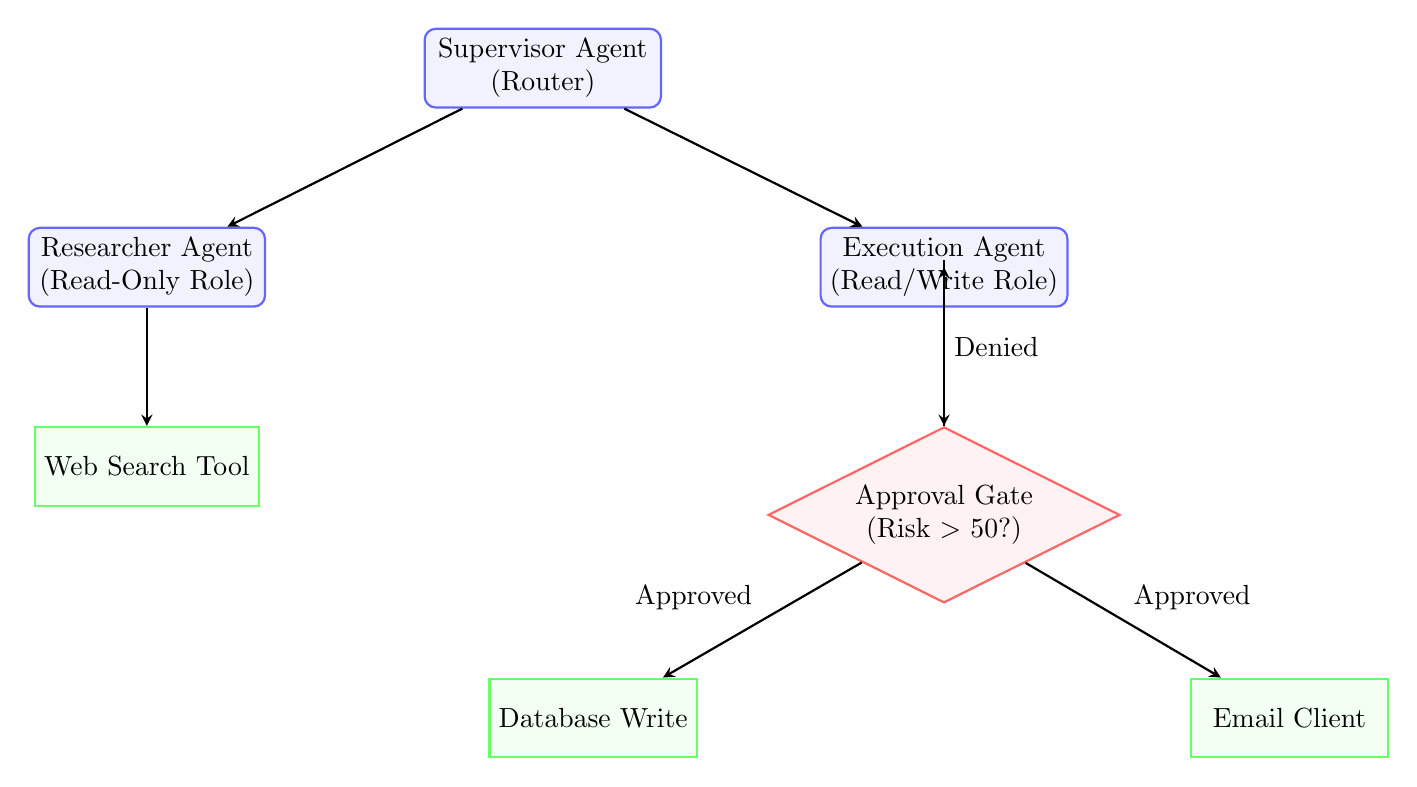
\begin{tikzpicture}[
    node distance=1.5cm and 2cm,
    agent/.style={rectangle, rounded corners, draw=blue!60, fill=blue!5, thick, minimum width=3cm, minimum height=1cm, align=center},
    tool/.style={rectangle, draw=green!60, fill=green!5, thick, minimum width=2.5cm, minimum height=1cm, align=center},
    gate/.style={diamond, draw=red!60, fill=red!5, thick, minimum width=2cm, minimum height=1cm, align=center, aspect=2},
    arrow/.style={thick,->,>=stealth}
]

% Nodes
\node[agent] (supervisor) {Supervisor Agent \\ (Router)};
\node[agent, below left=of supervisor] (researcher) {Researcher Agent \\ (Read-Only Role)};
\node[agent, below right=of supervisor] (executor) {Execution Agent \\ (Read/Write Role)};

\node[tool, below=of researcher] (search) {Web Search Tool};
\node[gate, below=of executor] (approval) {Approval Gate \\ (Risk $>$ 50?)};
\node[tool, below left=of approval] (db) {Database Write};
\node[tool, below right=of approval] (email) {Email Client};

% Arrows
\draw[arrow] (supervisor) -- (researcher);
\draw[arrow] (supervisor) -- (executor);

\draw[arrow] (researcher) -- (search);
\draw[arrow] (executor) -- (approval);

\draw[arrow] (approval) -- node[above left] {Approved} (db);
\draw[arrow] (approval) -- node[above right] {Approved} (email);
\draw[arrow] (approval) |- node[right, pos=0.25] {Denied} (executor);

\end{tikzpicture}
\end{center}

\vfill
\begin{center}\small
\textcopyright\ 2026 Sujeet Banerjee. All rights reserved.\\
Agentic AI Bootcamp -- Educational material.
\end{center}
\end{document}